%% This is an example first chapter.  You should put chapter/appendix that you
%% write into a separate file, and add a line \include{yourfilename} to
%% main.tex, where `yourfilename.tex' is the name of the chapter/appendix file.
%% You can process specific files by typing their names in at the 
%% \files=
%% prompt when you run the file main.tex through LaTeX.
\chapter{Conclusions}

With $B^0_s$ and $B^+$ measurements in PbPb collision, we can study beauty hadrochemistry and answer questions raised in Section 2.7.

\section{pp Reference and Theoretical Models}

Because our fully reconstructed B-meson analysis in pp as the reference is still ongoing, in order to understand our PbPb data, we need to add the B-meson pp measurements from other experiments at the LHC. The follow list the pp references we use to compare our PbPb measurement

\textbf{LHCb 7 TeV pp result at $2 < |y| < 5$:} This reference is chosen because it is one of the latest $B^0_s/B^+$ measurement with energy is closest to the 5.02 TeV in our analysis \ref{LHCbFF} . The original results is on the efficiency corrected yield ratio $\mathcal{R} = \frac{N(B^0_s \rightarrow J/\psi \phi)}{N(B^+ \rightarrow J/\psi K^+)} \cdot \frac{\epsilon(B^+ \rightarrow J/\psi K^+)}{\epsilon(B^0_s \rightarrow J/\psi \phi)}$ \cite{LHCbFF}. We scale $\mathcal{R}$ by the branching ratio of $B^0_s \rightarrow J/\psi \phi \rightarrow \mu^+\mu^- K^+ K^-$ to $B^+ \rightarrow J/\psi K^+ \rightarrow \mu^+\mu^- K^+$ and make them to be the same quantity as our $B^0_s/B^+$ measurement.

\textbf{ATLAS 7 TeV pp results at $|y| < 2.5$:}  \ref{ATLASPPRef} 


LHCb and ATLAS at different rapidity ranges. Since the rapidity dependence is not significant in $B^0_s/B^+$ ratio as demonstrated in Figure \ref{} from the LHCb publication \ref{}, assuming it is also insignificant in PbPb, we can use the pp reference at different rapidity ranges as references in our $B^0_s/B^+$ measurement

In addition to the pp reference, we also include the prediction from TAMU (labelled as ``PbPb: TAMU'' in orange), Cao, Sun, Ko (labelled as ``PbPb: Langevin'' in green), and (labelled as) which have been introduced in Section 1. Here we summarize 

Figure \ref{FinalResults} show the comparison between our $B^0_s/B^+$ measurement with pp references and theoretical model calculations. 

\begin{figure}[hbtp]
\begin{center}
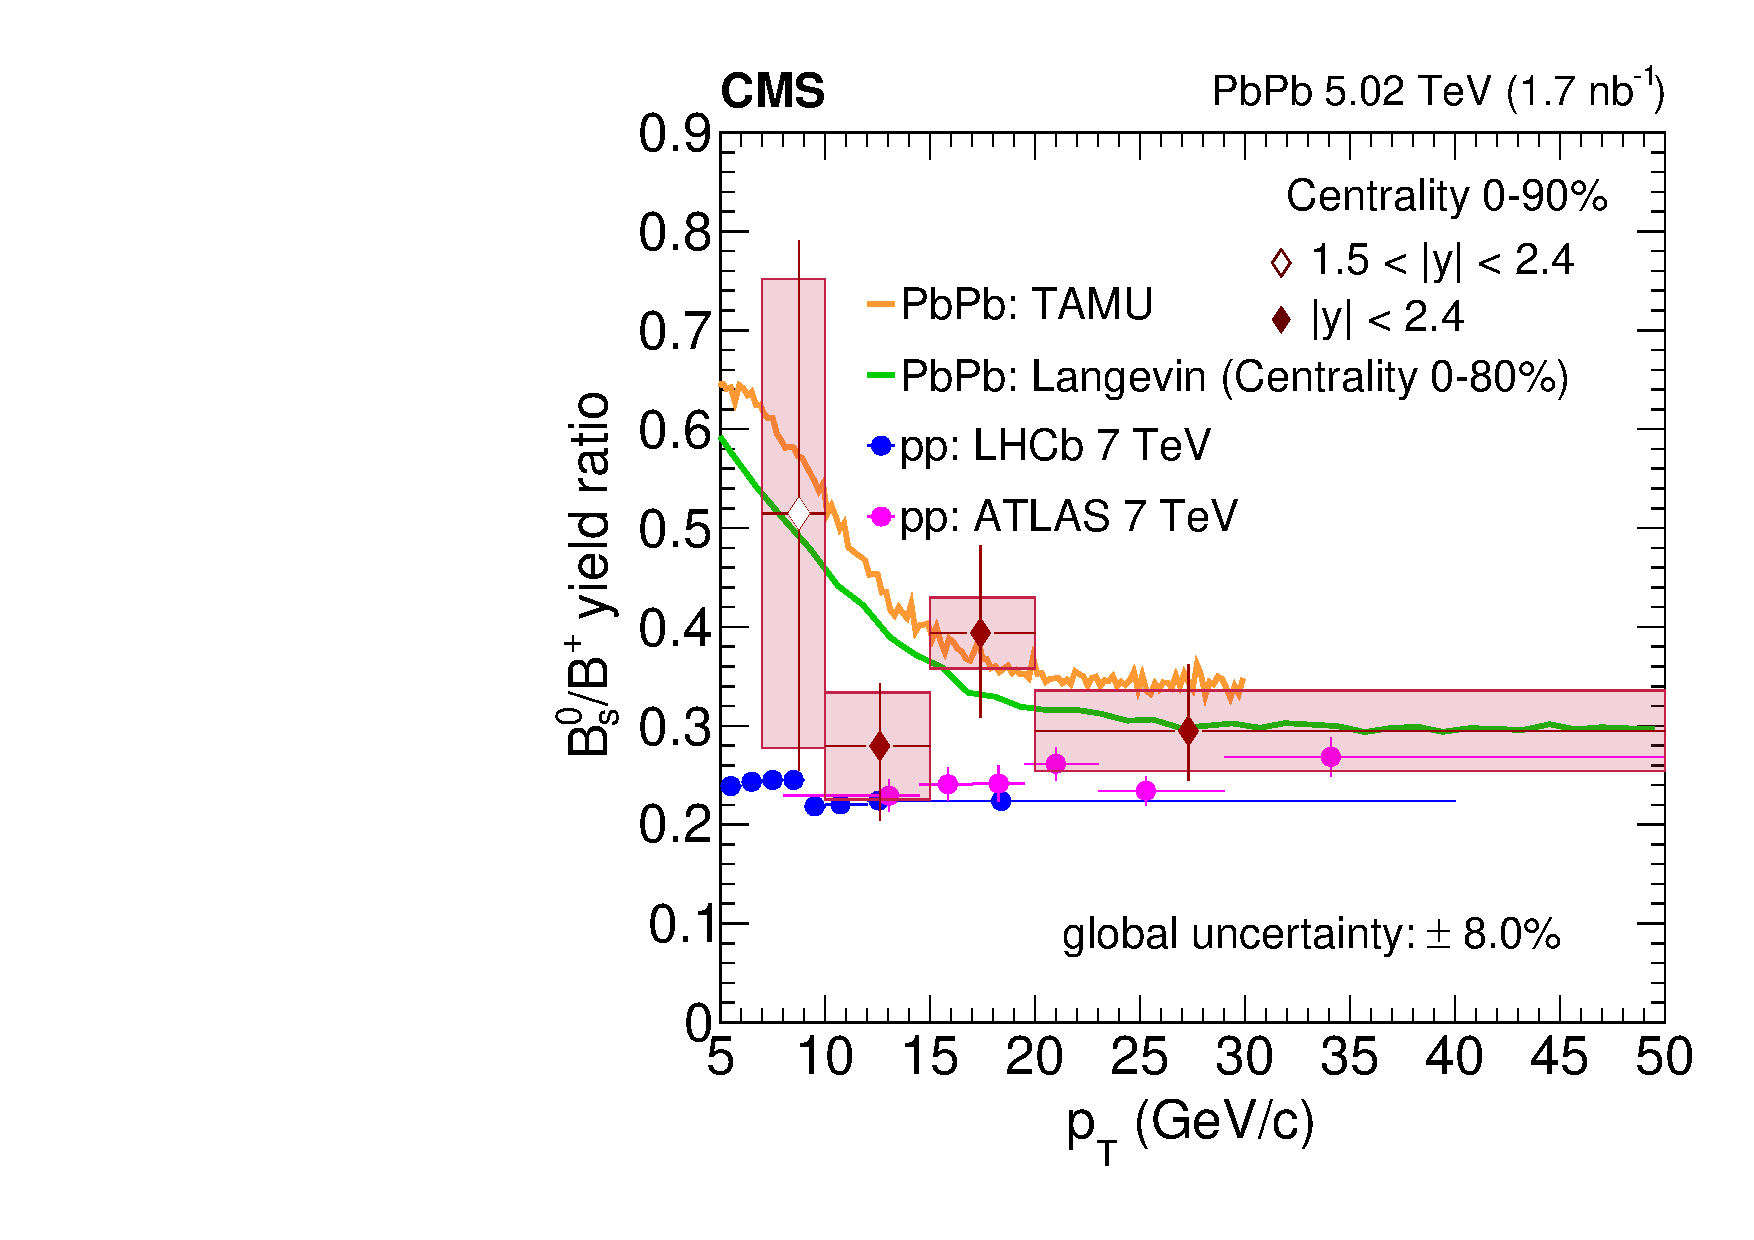
\includegraphics[width=0.48\textwidth]{Figures/Chapter6/ratio_vsPt_ref1_1.pdf}
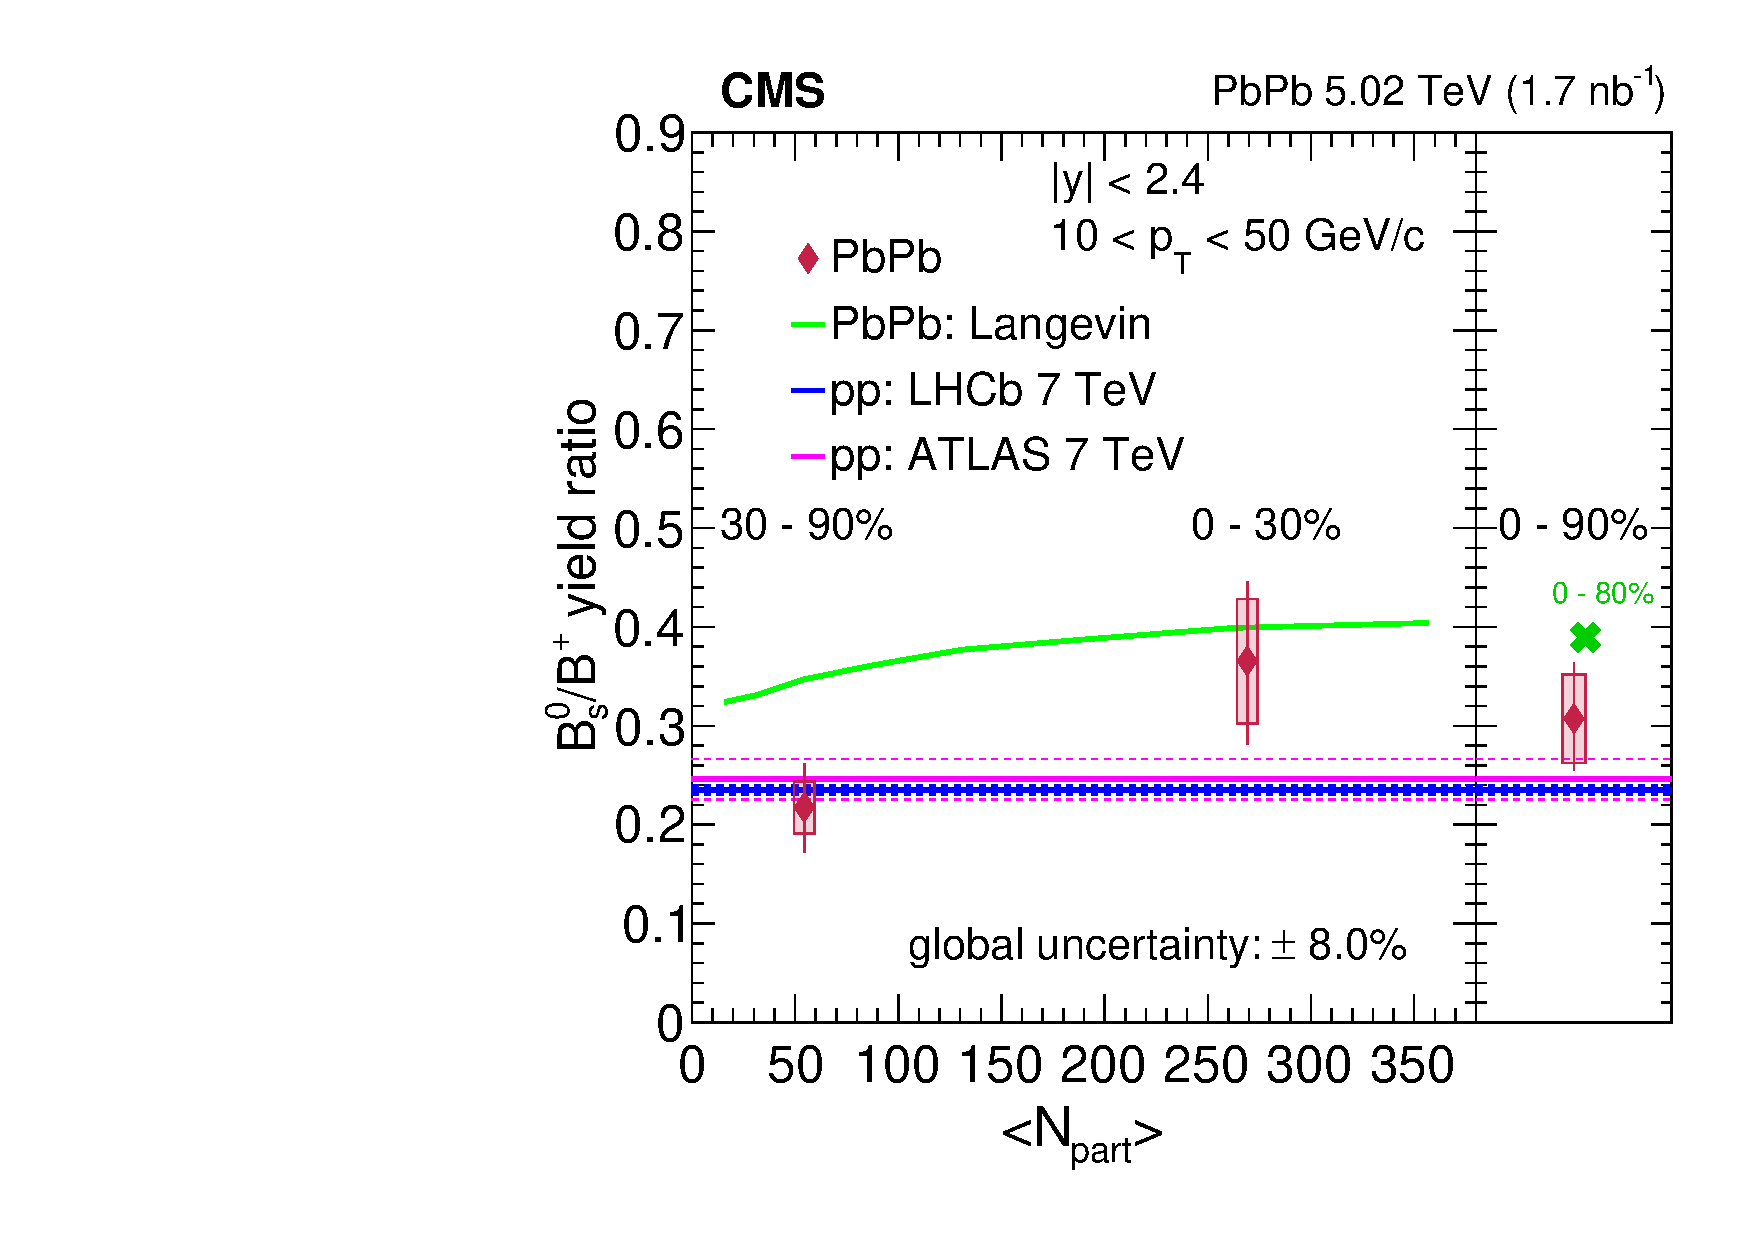
\includegraphics[width=0.48\textwidth]{Figures/Chapter6/ratio_vsCent_ref1.pdf}
\caption{The fully reconstructed $B^0_s/B^+$ (left) and $B^0_s/B^+$ $R_{AA}$ ratio (right) as a function of $p_T$ using the 2015 CMS pp and PbPb datasets are shown above. Both plot include the ATLAS (magenta) and LHCb (blue) 7 TeV reference. The TAMU model (orange) has only $p_T$ dependent prediction plot on the left figure while the Cao, Sun, Ko model (green) has both $p_T$ and centrality predictions plotted on both figures.}
\label{FinalResults}
\end{center}
\end{figure}   
 

\section{Physics Messages Discussion}

Figure \ref{FinalResults} conveys a lot of information. We will discuss the physics message of our measurement through the comparison of our data with the pp references and theoretical model prediction

Lies above but with in about 1.5 sigma. not significant $p_T$ dependence. Agree reasonably well with both TAMU and Cao, Sun, Ko models. compatible with LHCb data

List all the point here

\textbf{Substantial Uncertainties at Low $p_T$:} Both statistical and systematic uncertainties of $B^0_s/B^+$ ratio is large in $7 < p_T < 10$ GeV/c. They come $B^0_s$. However, we know that the statistics of $B^0_s$ in the $p_T$ range 7 - 10 GeV/c is indeed very small. In fact, from FONLL calculation, we expect to get only about $B^0_s$ candidates. From our estimation, we expect only about 100. Unfortunately, some of the systematic uncertainties, for instance, the one due to finite MC simulation statistics, which contribute a lot (25\%) to the total systematic uncertainties (46\%) can be in principle further reduce. 

\textbf{No significant $p_T$ dependence:} According to the $B^0/B^+$ ratio as a function of B-meson $p_T$, apparently, there is no significant change of the central values above 10 GeV/c. For 7 - 10 GeV/c, the central value jumps from 0.28 up to 0.51. However, the uncertainties of the measurement is also large. Considering all the uncertainties, we do not observe significant $p_T$ dependence on the $B^0_s/B^+$ ratio.

\textbf{Good Agreement with theoretical models:} Comparing our data to the TAMU and Cao, Sun Ko model calculations, the $B^0_s/B^+$ vs $p_T$ data agree well with these two models. They both predict the trend of the central values of our data, which decreases and then approaches to flat values as $p_T$ increases. The TAMU model always lies above the Cao, Sun, Ko model because it only employs quark coalescence model in hadronization. In Cao, Sun, Ko model, fragmentation hadronization is also considered. 

However, we know that in the limit $p_T \rightarrow \infty$, the $B^0_s/B^+$ in PbPb collision will be very similar to pp since the fast moving beauty quark traverse through the medium within a very short time and is not likely to combine with any quarks in the medium. Hence, fragmentation haronization dominates for fast moving beauty quarks. 

In the centrality measurement, the Cao, Sun, Ko model prediction are also reasonably consistent to our for 0 - 30\% and 0 - 90\%. However, in the peripheral 30 - 90\% collisions, the Cao, Sun, Ko model has a lager $B^0_s/B+$ ratio compared to our data, which coincides with the pp reference.  


\textbf{Compatible to pp references:} While the center $B^0_s/B^+$ data generally lies above the pp reference, 
 

\section{Conclusions}


\textbf{Pure fragmentation model is not enough to describe our data:} We can see that quark coalescence effect must be there because our data lies systematically above the pp reference. Looking at the most central collision from 0 - 30 \%, the $B^0_s/B^+$ ratio is about 1.5$\sigma$ above the LHCb pp reference. 

\textbf{Inconclusive no significant $p_T$ dependence}, more precise measurement needed 


%The $B^0_s$ and $B^+$ mesons are studied with the CMS detector at the LHC via the reconstruction of the exclusive hadronic decay channels B\ and \Bplusdecayall.  The measurements are performed within the \PB\ mesons' fiducial region given by transverse momentum $\pt>10\GeVc$ for rapidity $\abs{y}<1.5$  and  $7<\pt<50\GeVc \,$ for $1.5<\abs{y}<2.4$. The first observation of the \PBzs\ meson in nucleus-nucleus collisions, with a statistical significance well surpassing five standard deviations, is attained. The production yields of \PBzs\ and \PBp\ mesons, scaled by the nuclear overlap function \TAA and the number of minimum bias events \NMB, in lead-lead (\PbPb) collisions at a center-of-mass energy of $5.02\TeV$ per nucleon pair are presented as functions of the meson \pt\ and for the first time of the event centrality. These results extend, and are compatible with, those previously reported by the CMS Collaboration~\cite{BsPbPbCMS,BpPbPbCMS}, and are based on a three-fold larger \PbPb\ data sample. The ratio of production yields of the two mesons in \PbPb\ collisions is determined and it is found to be statistically compatible with the corresponding ratio in proton-proton (\pp) collisions. The further investigation of possible hints of an enhancement of the ratio in \PbPb, relative to \pp, collisions will benefit from more precise \PbPb\ and \pp\ reference data taken at the same collision energy per nucleon. The larger \PbPb\ data sets that should be accumulated in upcoming high-luminosity LHC heavy ion runs will provide greater precision and could help to further characterize the mechanisms of beauty hadronization in heavy ion collisions.






We have performed the 
Conclude the message. Draw final based on the points. Answer question post previously

More precise measurement. 



\section{Future Outlooks}

As mentioned previous, current results still limited. It would also be great . Figure \ref{} shows our ongoing analysis of fully reconstructed $B^0_s$, $B^+$, and $B^0$ via the decay channels of 


Very clear B-meson signals have been observed. The estimated significance are all greater 4. With these signals, we can perform measurement on $B^+$ cross section in pp collisions down to 0 $p_T$, which allows us to perform measurement of inclusive beauty production cross section. In addition, we will also be able to measure $B^0_s/B^+$ ratio down to 3 GeV/c. Also, according to the multiplicity studies, we can also $B^0_s/B^+$ as a function of multiplicity up to 150, which also help us answer questions raised in Chapter 2. 

In the era of LHC Run 3 and HL-LHC, much more statistics will be collected to perform measurement on fully reconstructed $B^+_c$ and $\Lambda_b$. With the potential update of CMS MTD, we can good performance of PID for particle momentum from to GeV/c, which allow us to measure down to very low $p_T$. 

Finally, with the sPHENIX experiment at RHIC taking data in 2023, we can also fully reconstruct b hadrons at RHIC energy to study a QGP medium at a lower temperature and higher baryon chemical potential. The beauty measurement at RHIC will be complementary to the measurements at the LHC. Together, these will help determine heavy quark diffusion coefficient with different temperature, constrain the fundamental property of QGP $\eta/s$, and probe the inner workings of QGP. To fully explore open heavy flavor physics and understand the inner workings of QGP, lots of challenges and opportunities are awaiting. A bright and exciting future of heavy flavor physics in heavy-ion collision will be forthcoming.



